
\subsection*{3.2 Circles}
Circles are fundamental shapes in geometry and have unique properties and theorems associated with them. Below are key concepts and theorems related to circles.

\textbf{Key Concepts:}
\begin{itemize}
	\item \textbf{Radius and Diameter:} The radius is the distance from the center of the circle to any point on its circumference. The diameter is twice the radius.
	\item \textbf{Circumference:} The perimeter of a circle is given by the formula:
	\[
	C = 2\pi r,
	\]
	where $r$ is the radius.
	\item \textbf{Area:} The area of a circle is given by:
	\[
	A = \pi r^2.
	\]
	\item \textbf{Tangent:} A tangent to a circle is a line that touches the circle at exactly one point. The radius at the point of tangency is perpendicular to the tangent.
	\item \textbf{Chord:} A chord is a line segment with endpoints on the circle. The perpendicular from the center to a chord bisects the chord.
	\item \textbf{Arc and Sector:} An arc is a part of the circumference, and a sector is the region enclosed by two radii and an arc.
	\begin{center}
		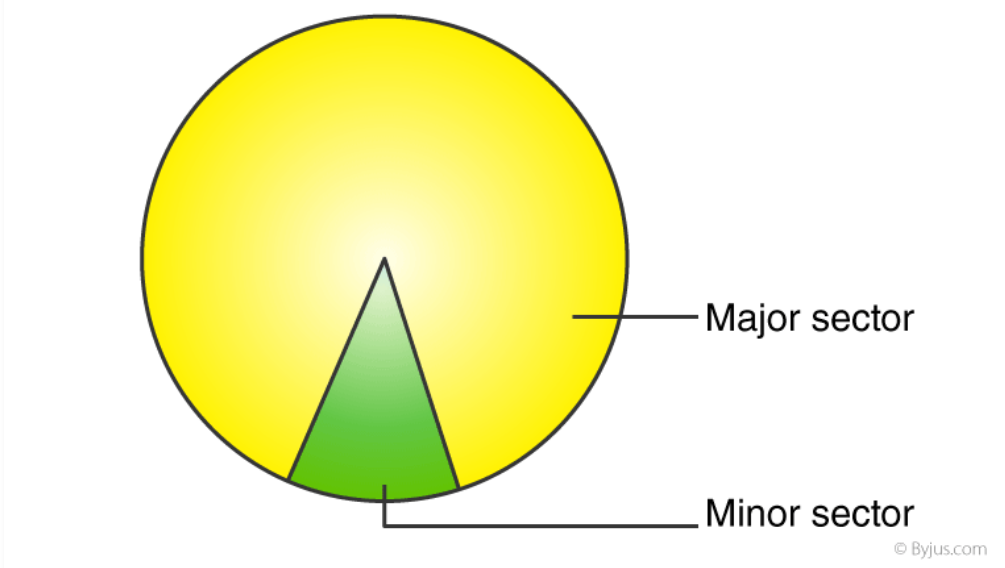
\includegraphics[width=0.6\textwidth]{3.3.png}
	\end{center}
	\begin{center}
		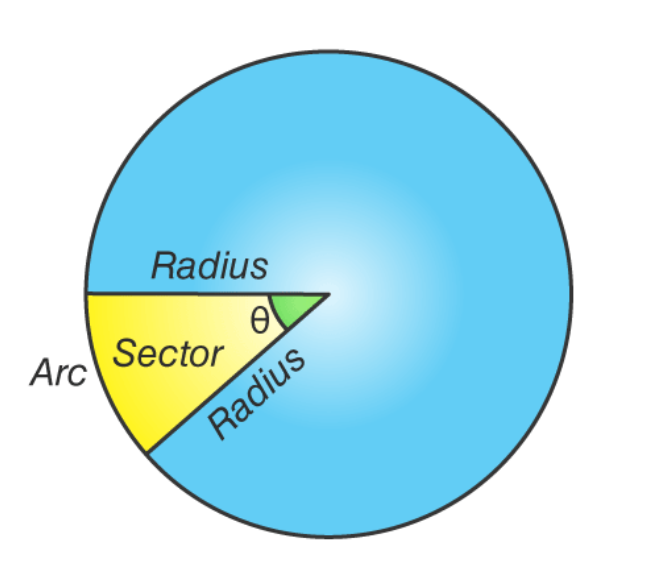
\includegraphics[width=0.6\textwidth]{3.4.png}
	\end{center}
	\item \textbf{Area of an sector and Arc length:} 
	\[
	\text{Area of Sector} = \frac{\theta}{360^\circ} \times \pi r^2,
	\]
	\[
	\text{Arc Length} = \frac{\theta}{360^\circ} \times 2\pi r,
	\]
	where $\theta$ is the central angle in degrees and $r$ is the radius of the circle.
	
\end{itemize}

\textbf{Circle Theorems:}
\begin{itemize}
	\item \textbf{Angle at the Center:} The angle subtended by an arc at the center of a circle is twice the angle subtended at any point on the circumference.
	\item \textbf{Angle in a Semicircle:} The angle subtended by a diameter at the circumference is a right angle.
	\item \textbf{Cyclic Quadrilateral:} The opposite angles of a cyclic quadrilateral (a quadrilateral inscribed in a circle) are supplementary.
	\item \textbf{Tangent-Secant Theorem:} If a tangent and a secant are drawn from an external point, then the square of the length of the tangent is equal to the product of the secant's external and total lengths.
	
	\begin{center}
		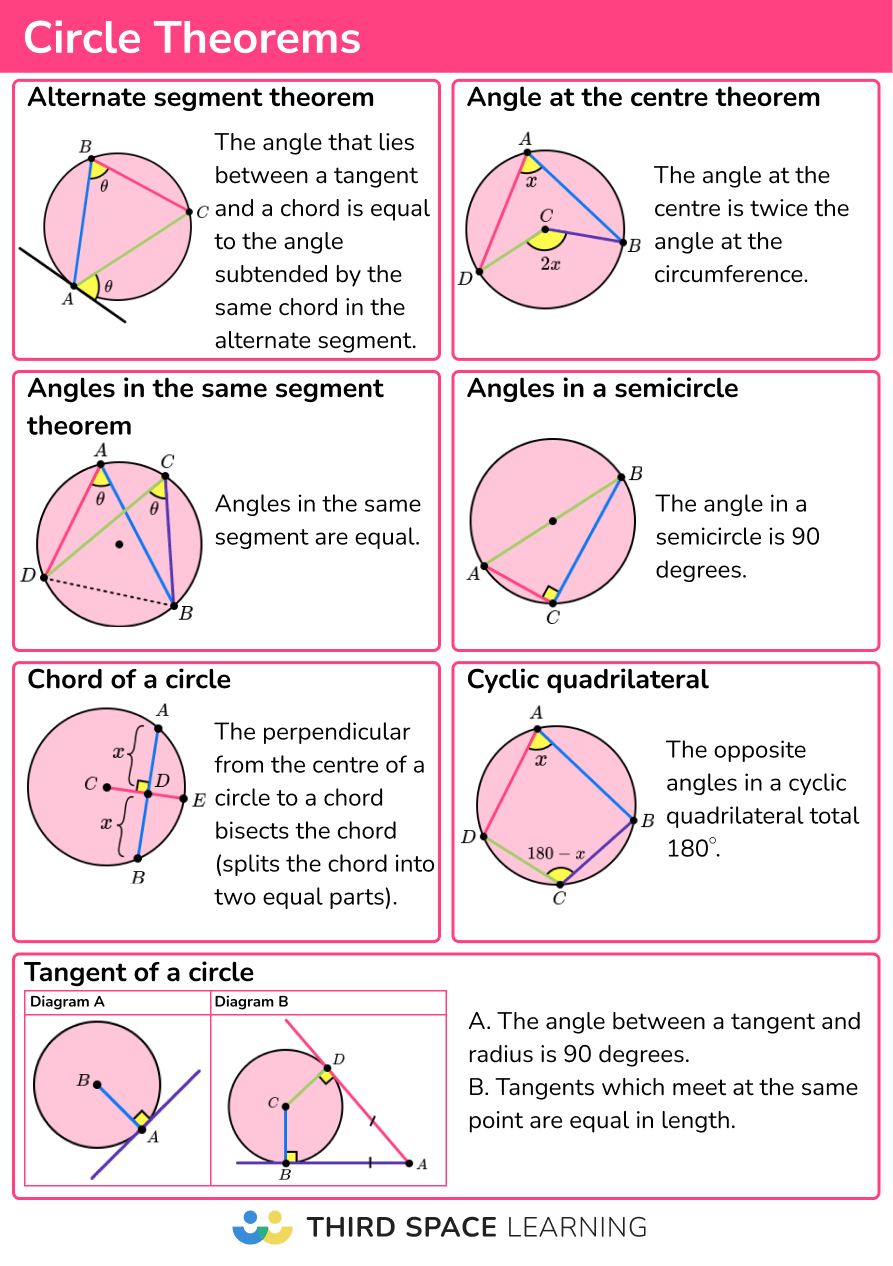
\includegraphics[width=0.6\textwidth]{3.5.png}
	\end{center}
\end{itemize}

\textbf{Examples:}

\begin{flushleft}
	\textbf{Example 1: Find the circumference of a circle with radius 7 cm.}
	
	\vspace{0.5cm}
	\textbf{Solution:}
	\vspace{0.5cm}
	
	Use the formula for circumference:
	\[
	C = 2\pi r = 2 \times \pi \times 7 = 14\pi \approx 43.98 \text{ cm}.
	\]
	Therefore, the circumference is approximately $43.98$ cm.
\end{flushleft}

\begin{flushleft}
	\textbf{Example 2: A chord of a circle is 12 cm long, and its distance from the center is 5 cm. Find the radius of the circle.}
	
	\vspace{0.5cm}
	\textbf{Solution:}
	\vspace{0.5cm}
	
	Let the radius be $r$. Using the Pythagoras theorem in the triangle formed by the radius, half the chord, and the perpendicular distance:
	\[
	r^2 = 6^2 + 5^2 = 36 + 25 = 61.
	\]
	\[
	r = \sqrt{61} \approx 7.81 \text{ cm}.
	\]
	Therefore, the radius of the circle is approximately $7.81$ cm.
\end{flushleft}

\begin{flushleft}
	\textbf{Example 3: Prove that the angle subtended by a diameter at the circumference is a right angle.}
	
	\vspace{0.5cm}
	\textbf{Solution:}
	\vspace{0.5cm}
	
	Let $ABC$ be a triangle inscribed in a circle, where $AB$ is the diameter. By the angle at the center theorem:
	\[
	\text{Angle at the center } \angle AOB = 180^\circ.
	\]
	\[
	\text{Angle at the circumference } \angle ACB = \frac{1}{2} \times 180^\circ = 90^\circ.
	\]
	Therefore, the angle subtended by a diameter is always a right angle.
\end{flushleft}

\begin{flushleft}
	\textbf{Example 4: Find the area of a sector with radius 6 cm and central angle $60^\circ$.}
	
	\vspace{0.5cm}
	\textbf{Solution:}
	\vspace{0.5cm}
	
	Use the formula for the area of a sector:
	\[
	A = \frac{\theta}{360^\circ} \times \pi r^2 = \frac{60^\circ}{360^\circ} \times \pi \times 6^2.
	\]
	Simplify:
	\[
	A = \frac{1}{6} \times \pi \times 36 = 6\pi \approx 18.85 \text{ cm}^2.
	\]
	Therefore, the area of the sector is approximately $18.85 \text{ cm}^2$.
\end{flushleft}

\begin{flushleft}
	\textbf{Example 5: In the diagram below, $O$ is the center of the circle $QRS$ and $\angle SQR = 28^\circ$. Find $\angle ORS$.}
	
	\vspace{0.5cm}
	\begin{center}
		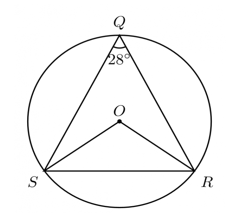
\includegraphics[width=0.6\textwidth]{3.6.png}
	\end{center}
	
	\textbf{Solution:}
	\vspace{0.5cm}
	
	Step 1: Recall the Circle Theorem for angles at the center and circumference:
	The angle subtended by an arc at the center of a circle is twice the angle subtended at the circumference by the same arc.
	
	Step 2: Identify the arc and the angles:
	- $\angle SQR$ is the angle subtended at the circumference by the arc $SR$.
	- $\angle SOR$ is the angle subtended at the center by the same arc.
	
	Step 3: Use the Circle Theorem:
	\[
	\angle SOR = 2 \times \angle SQR.
	\]
	
	Substitute $\angle SQR = 28^\circ$:
	\[
	\angle SOR = 2 \times 28^\circ = 56^\circ.
	\]
	
	Step 4: Find $\angle ORS$:
	Since $\triangle OSR$ is an isosceles triangle (radii $OS$ and $OR$ are equal), the base angles are equal:
	\[
	\angle ORS = \angle OSR = \frac{180^\circ - \angle SOR}{2}.
	\]
	
	Substitute $\angle SOR = 56^\circ$:
	\[
	\angle ORS = \frac{180^\circ - 56^\circ}{2} = \frac{124^\circ}{2} = 62^\circ.
	\]
	
	Therefore, $\angle ORS = 62^\circ$.
\end{flushleft}

